\setcounter{chapter}{1}
\setcounter{figure}{0}
\renewcommand\thechapter{\Alph{chapter}}

\chapter*{Додатки}\addcontentsline{toc}{chapter}{\MakeUppercase{Додатки}}

\centeredsection

\section*{Додаток А}\addcontentsline{toc}{section}{Додаток А}
\begin{center}
	\bfseries Зразки користувацького інтерфейсу Android-щоденника
\end{center}

\begin{figure}[H]
	\centering
	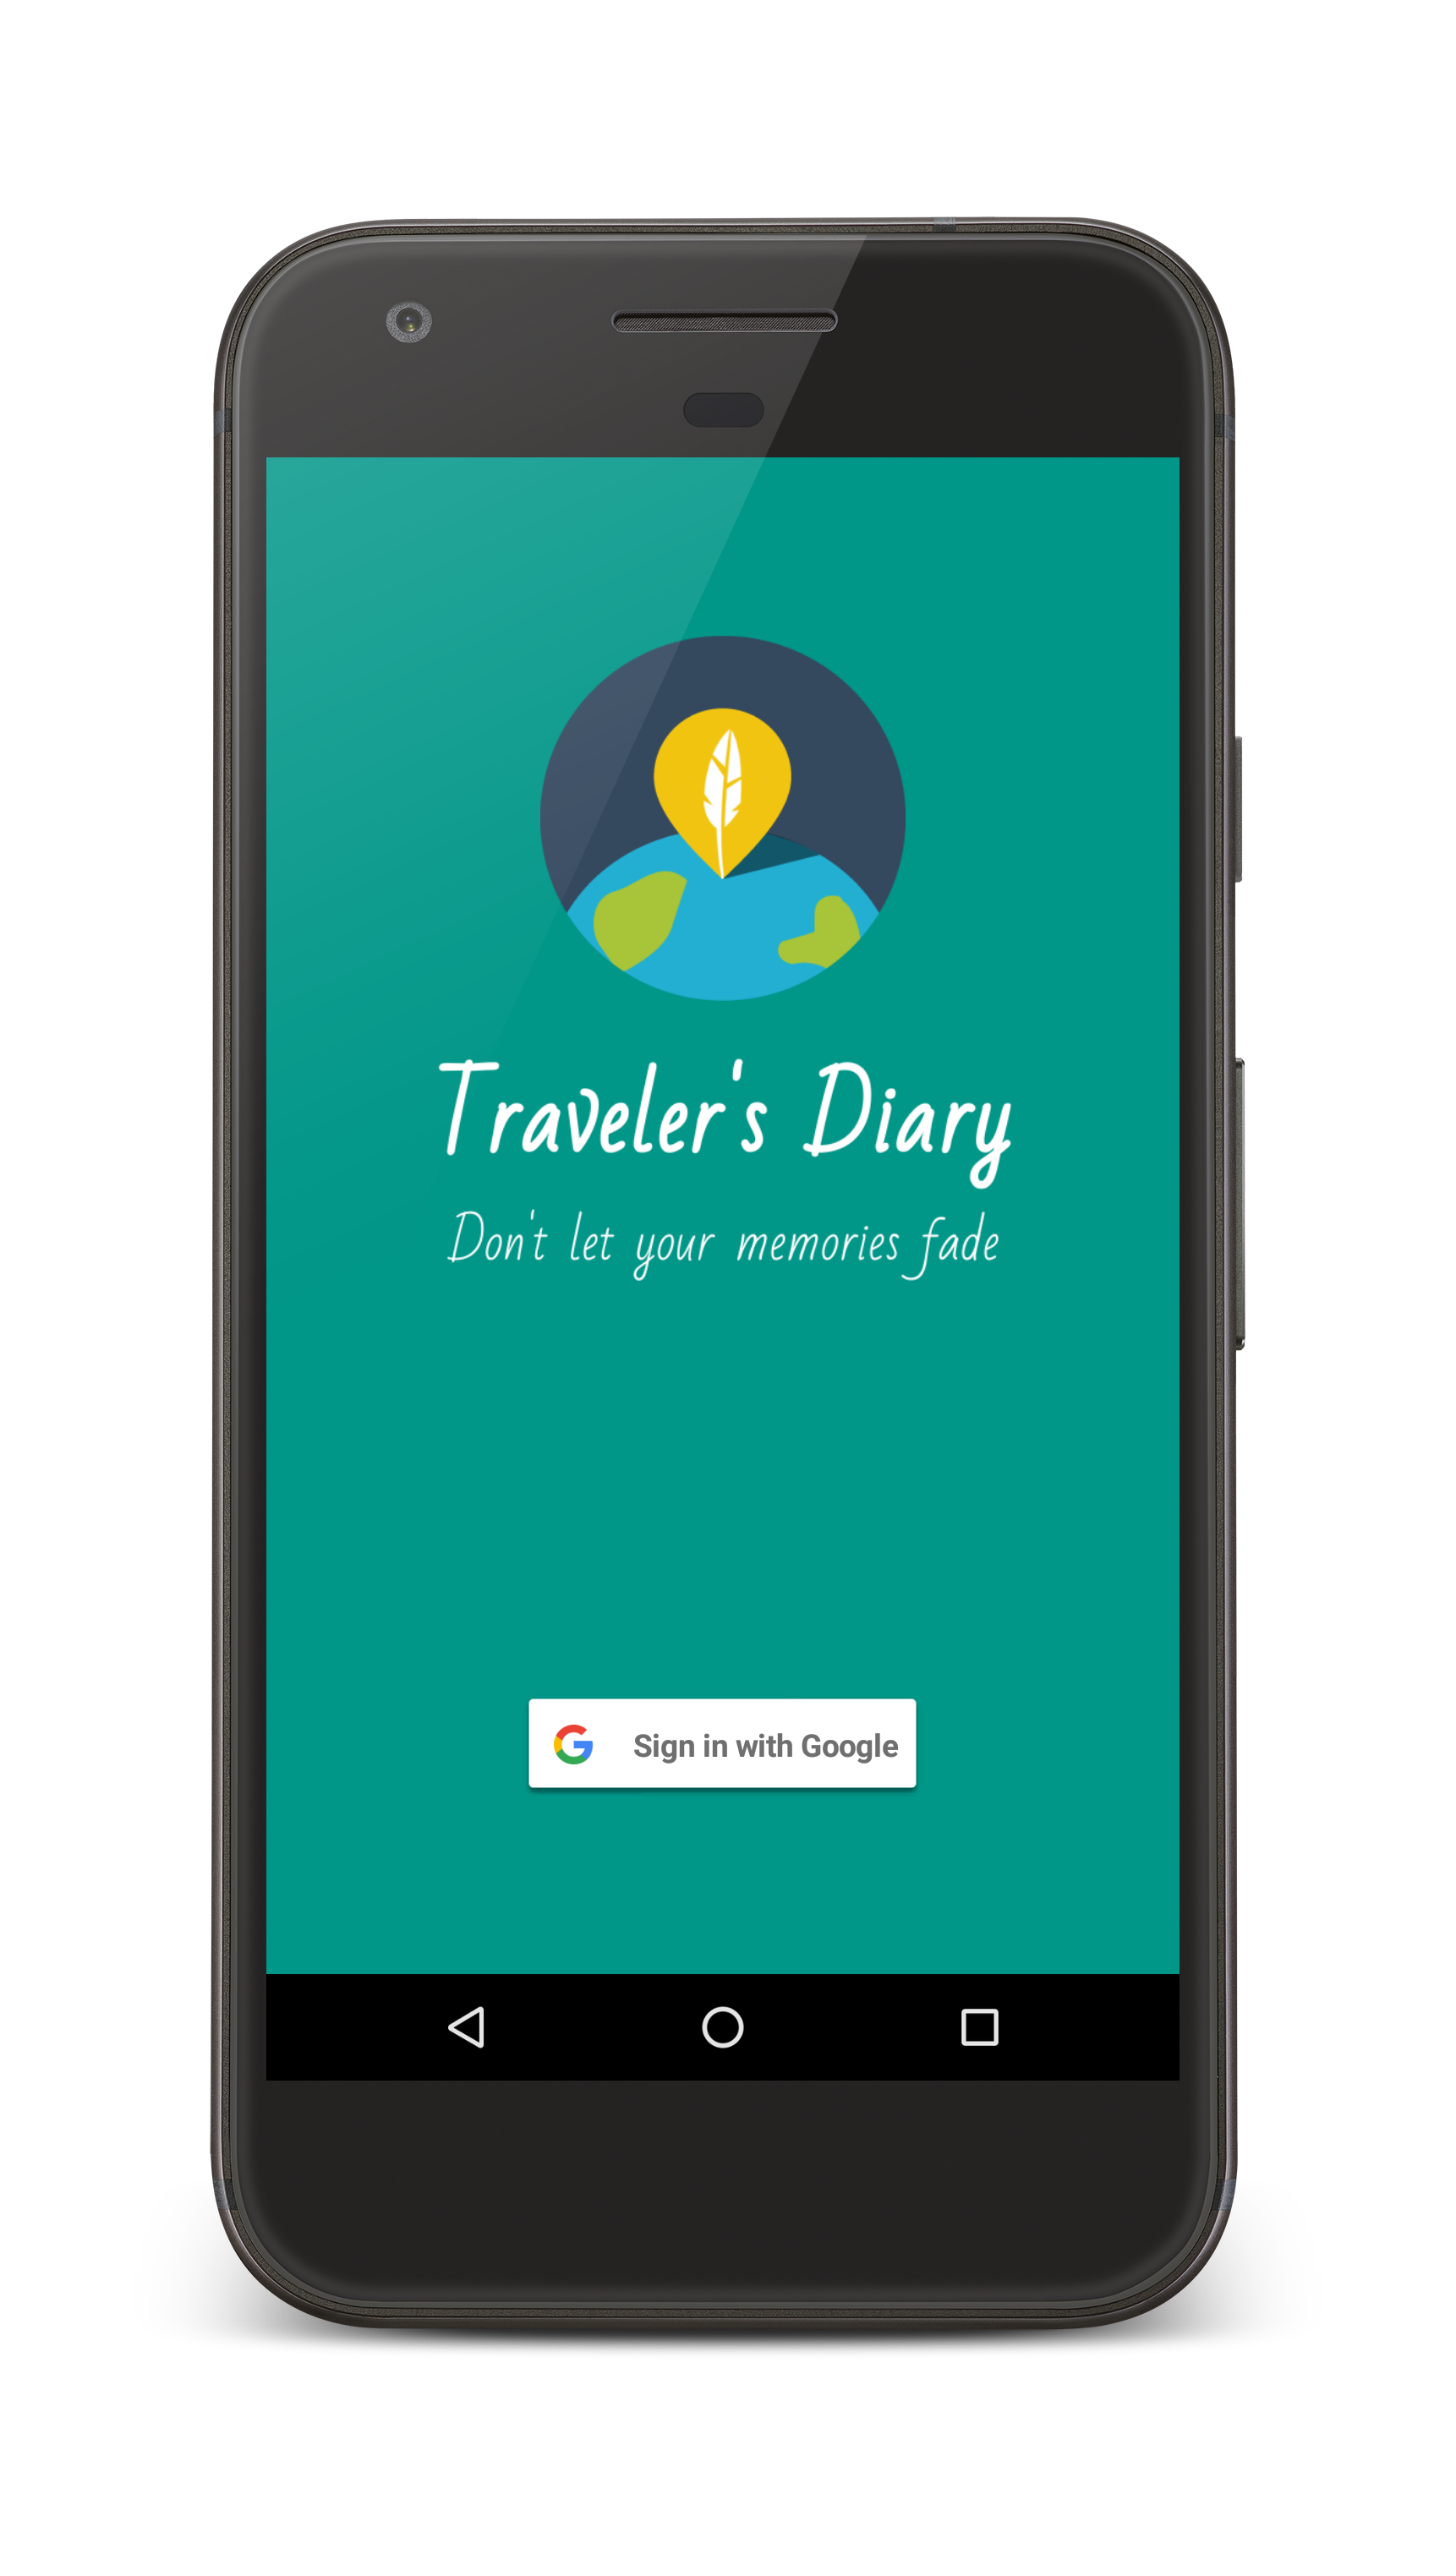
\includegraphics[width=0.6\textwidth]{auth_screen}
	\caption{Екран авторизації}
	\label{auth_screen}
\end{figure}

\begin{figure}[H]
	\centering
	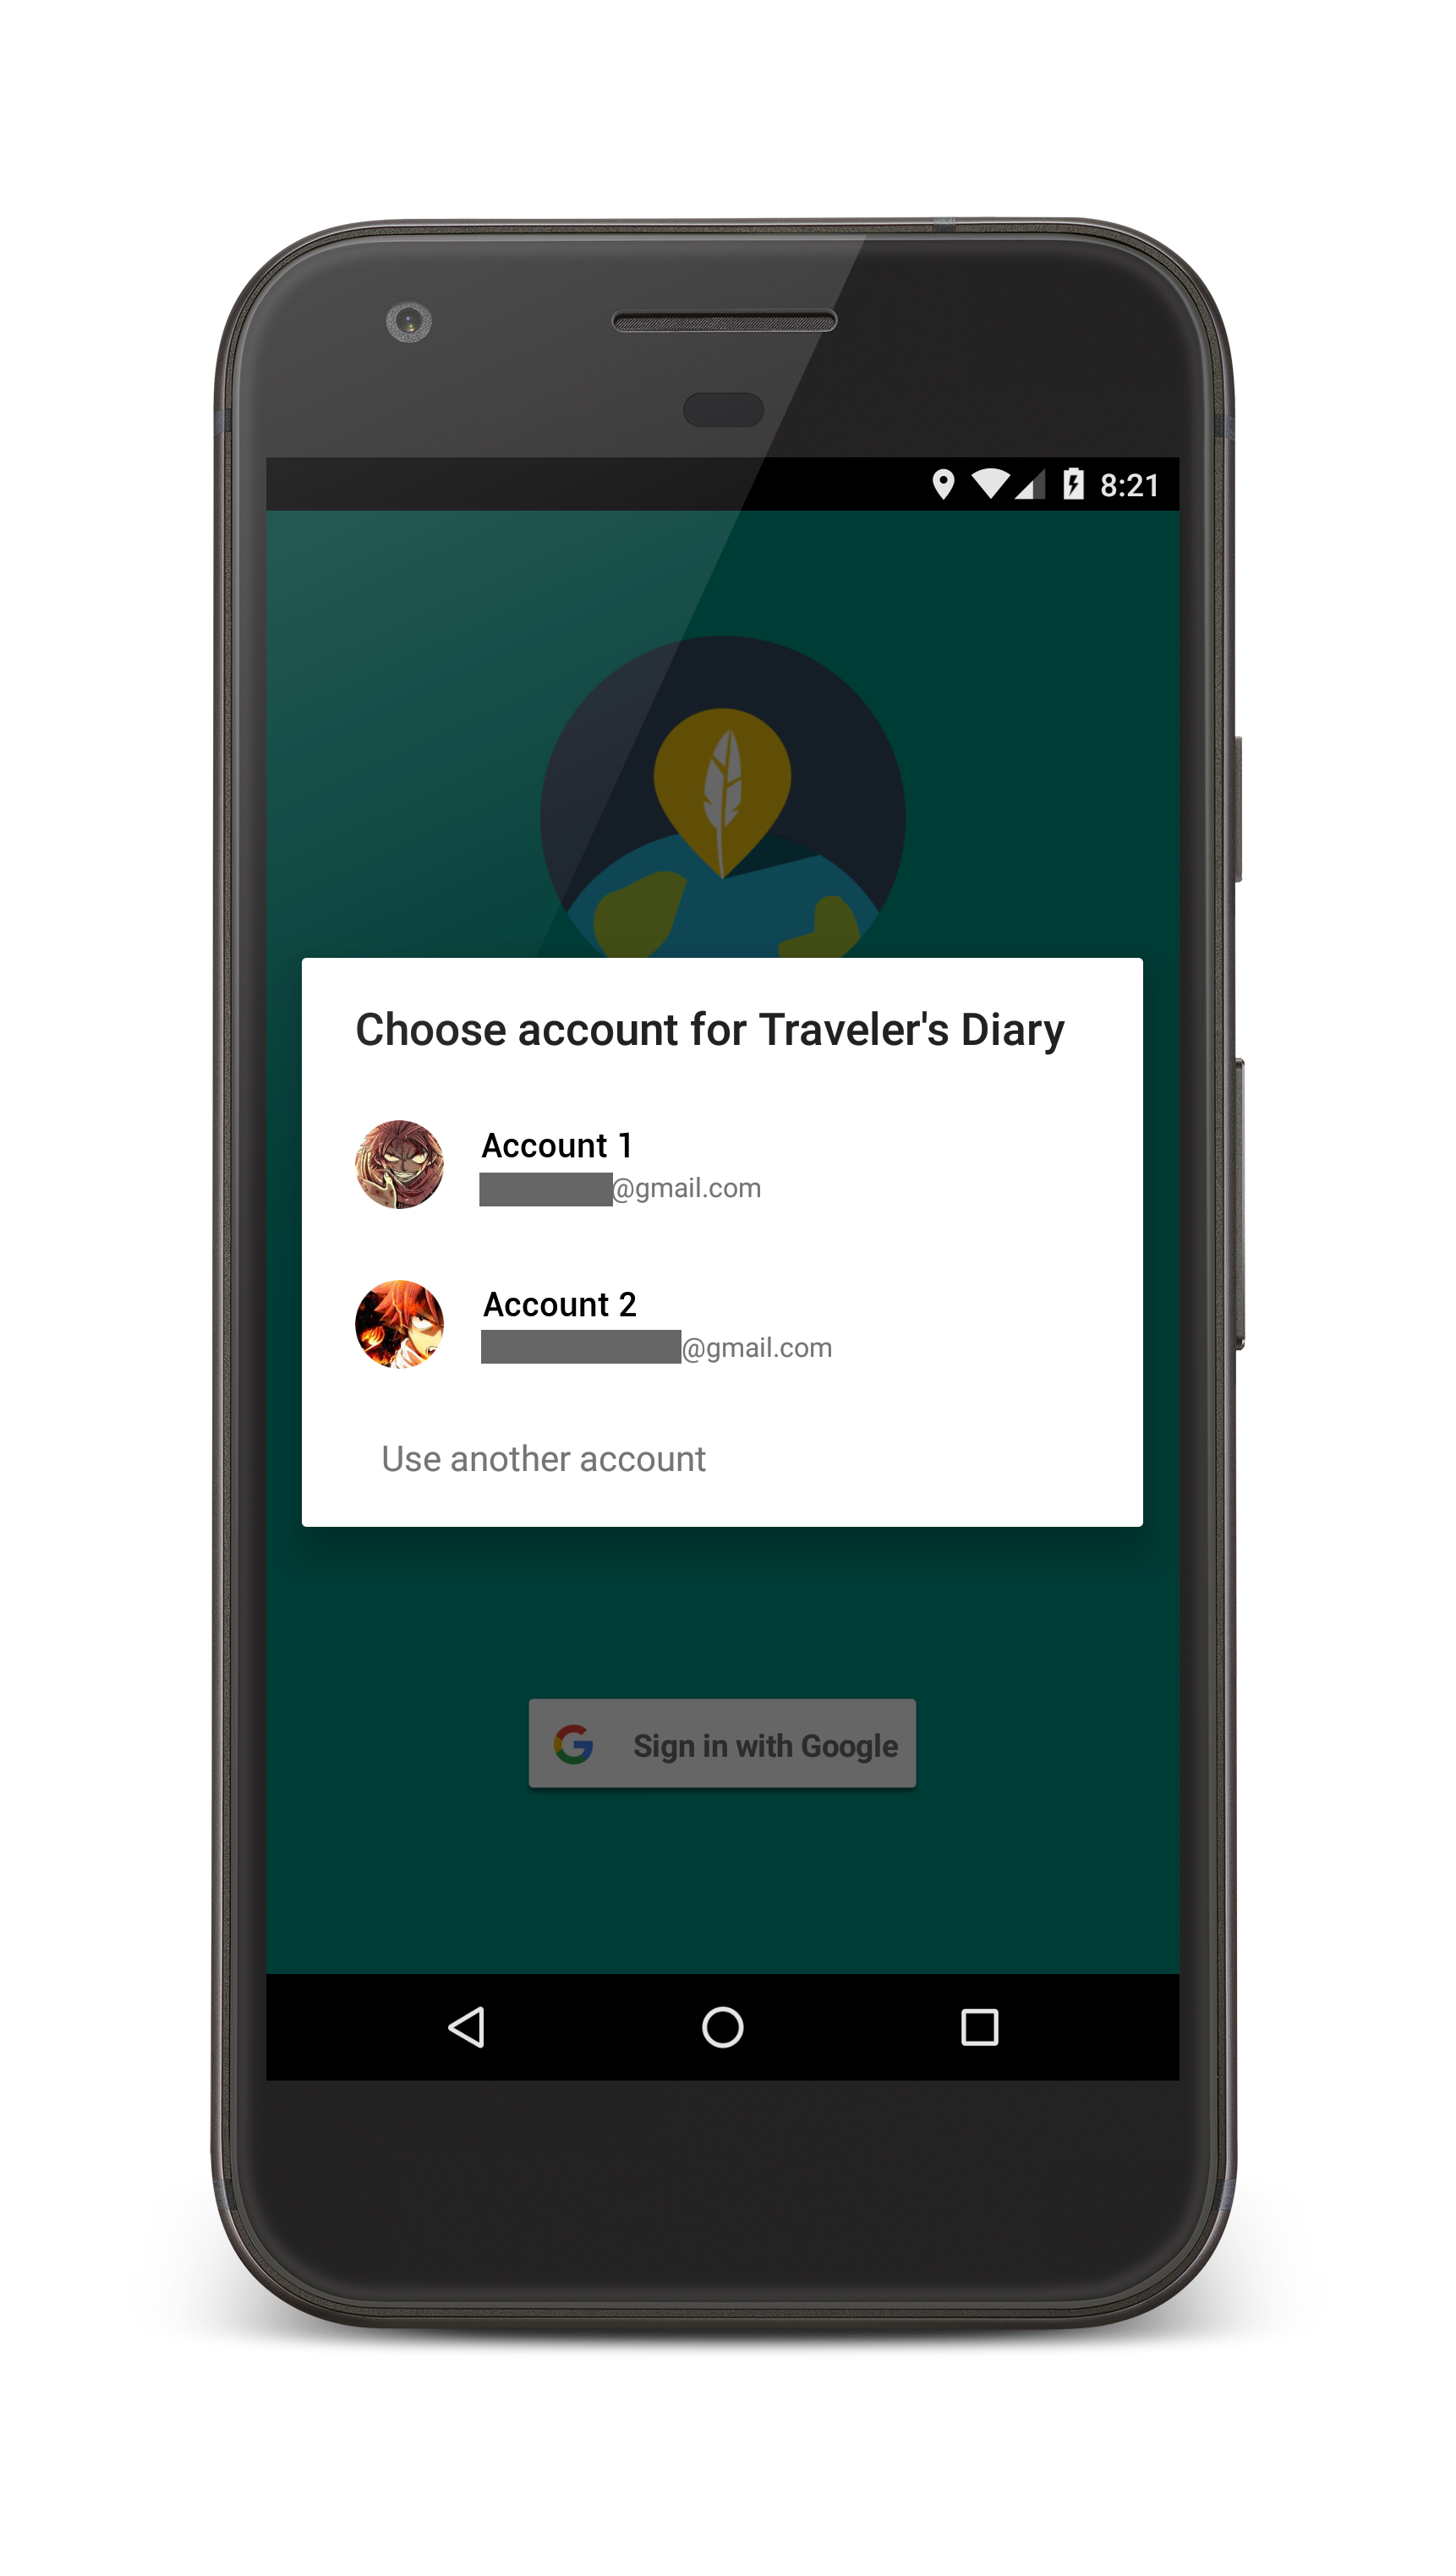
\includegraphics[width=0.75\textwidth]{choose_screen}
	\caption{Екран вибору Google акаунта}
	\label{choose_screen}
\end{figure}

\begin{figure}[H]
	\centering
	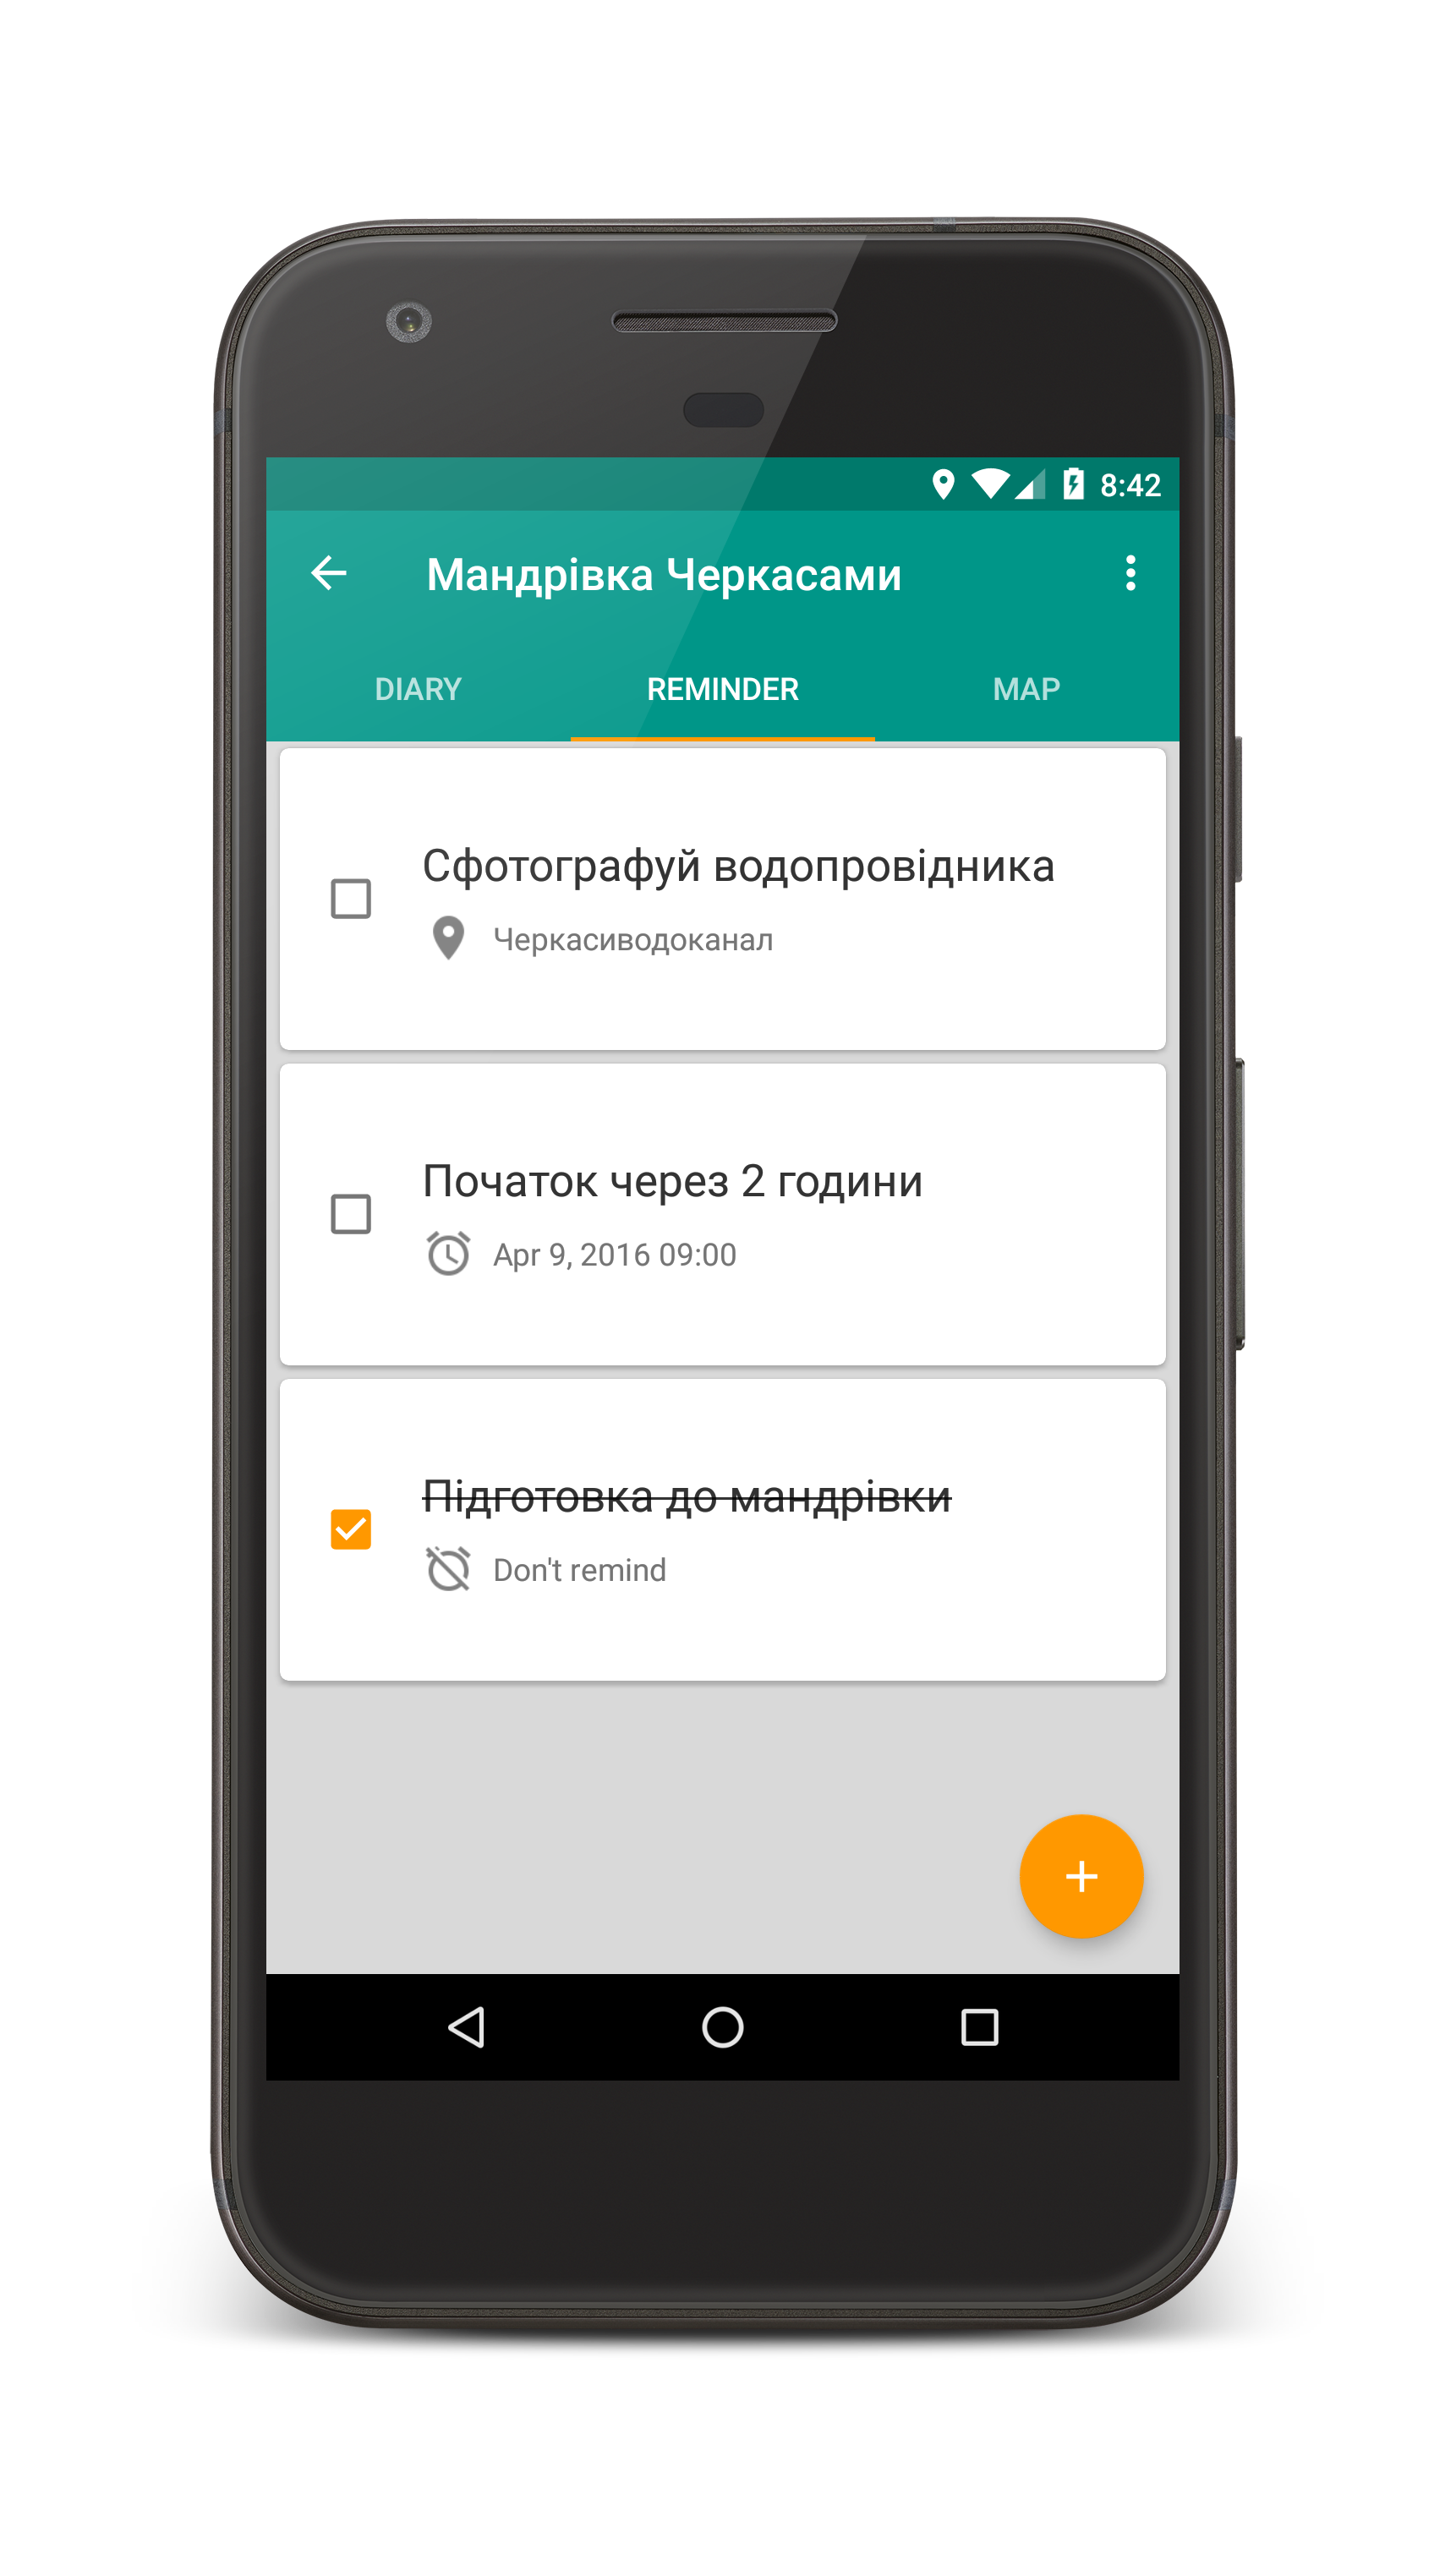
\includegraphics[width=0.75\textwidth]{reminderlist_screen}
	\caption{Екран списку записів планувальника}
	\label{reminder_list_screen}
\end{figure}

\begin{figure}[H]
	\centering
	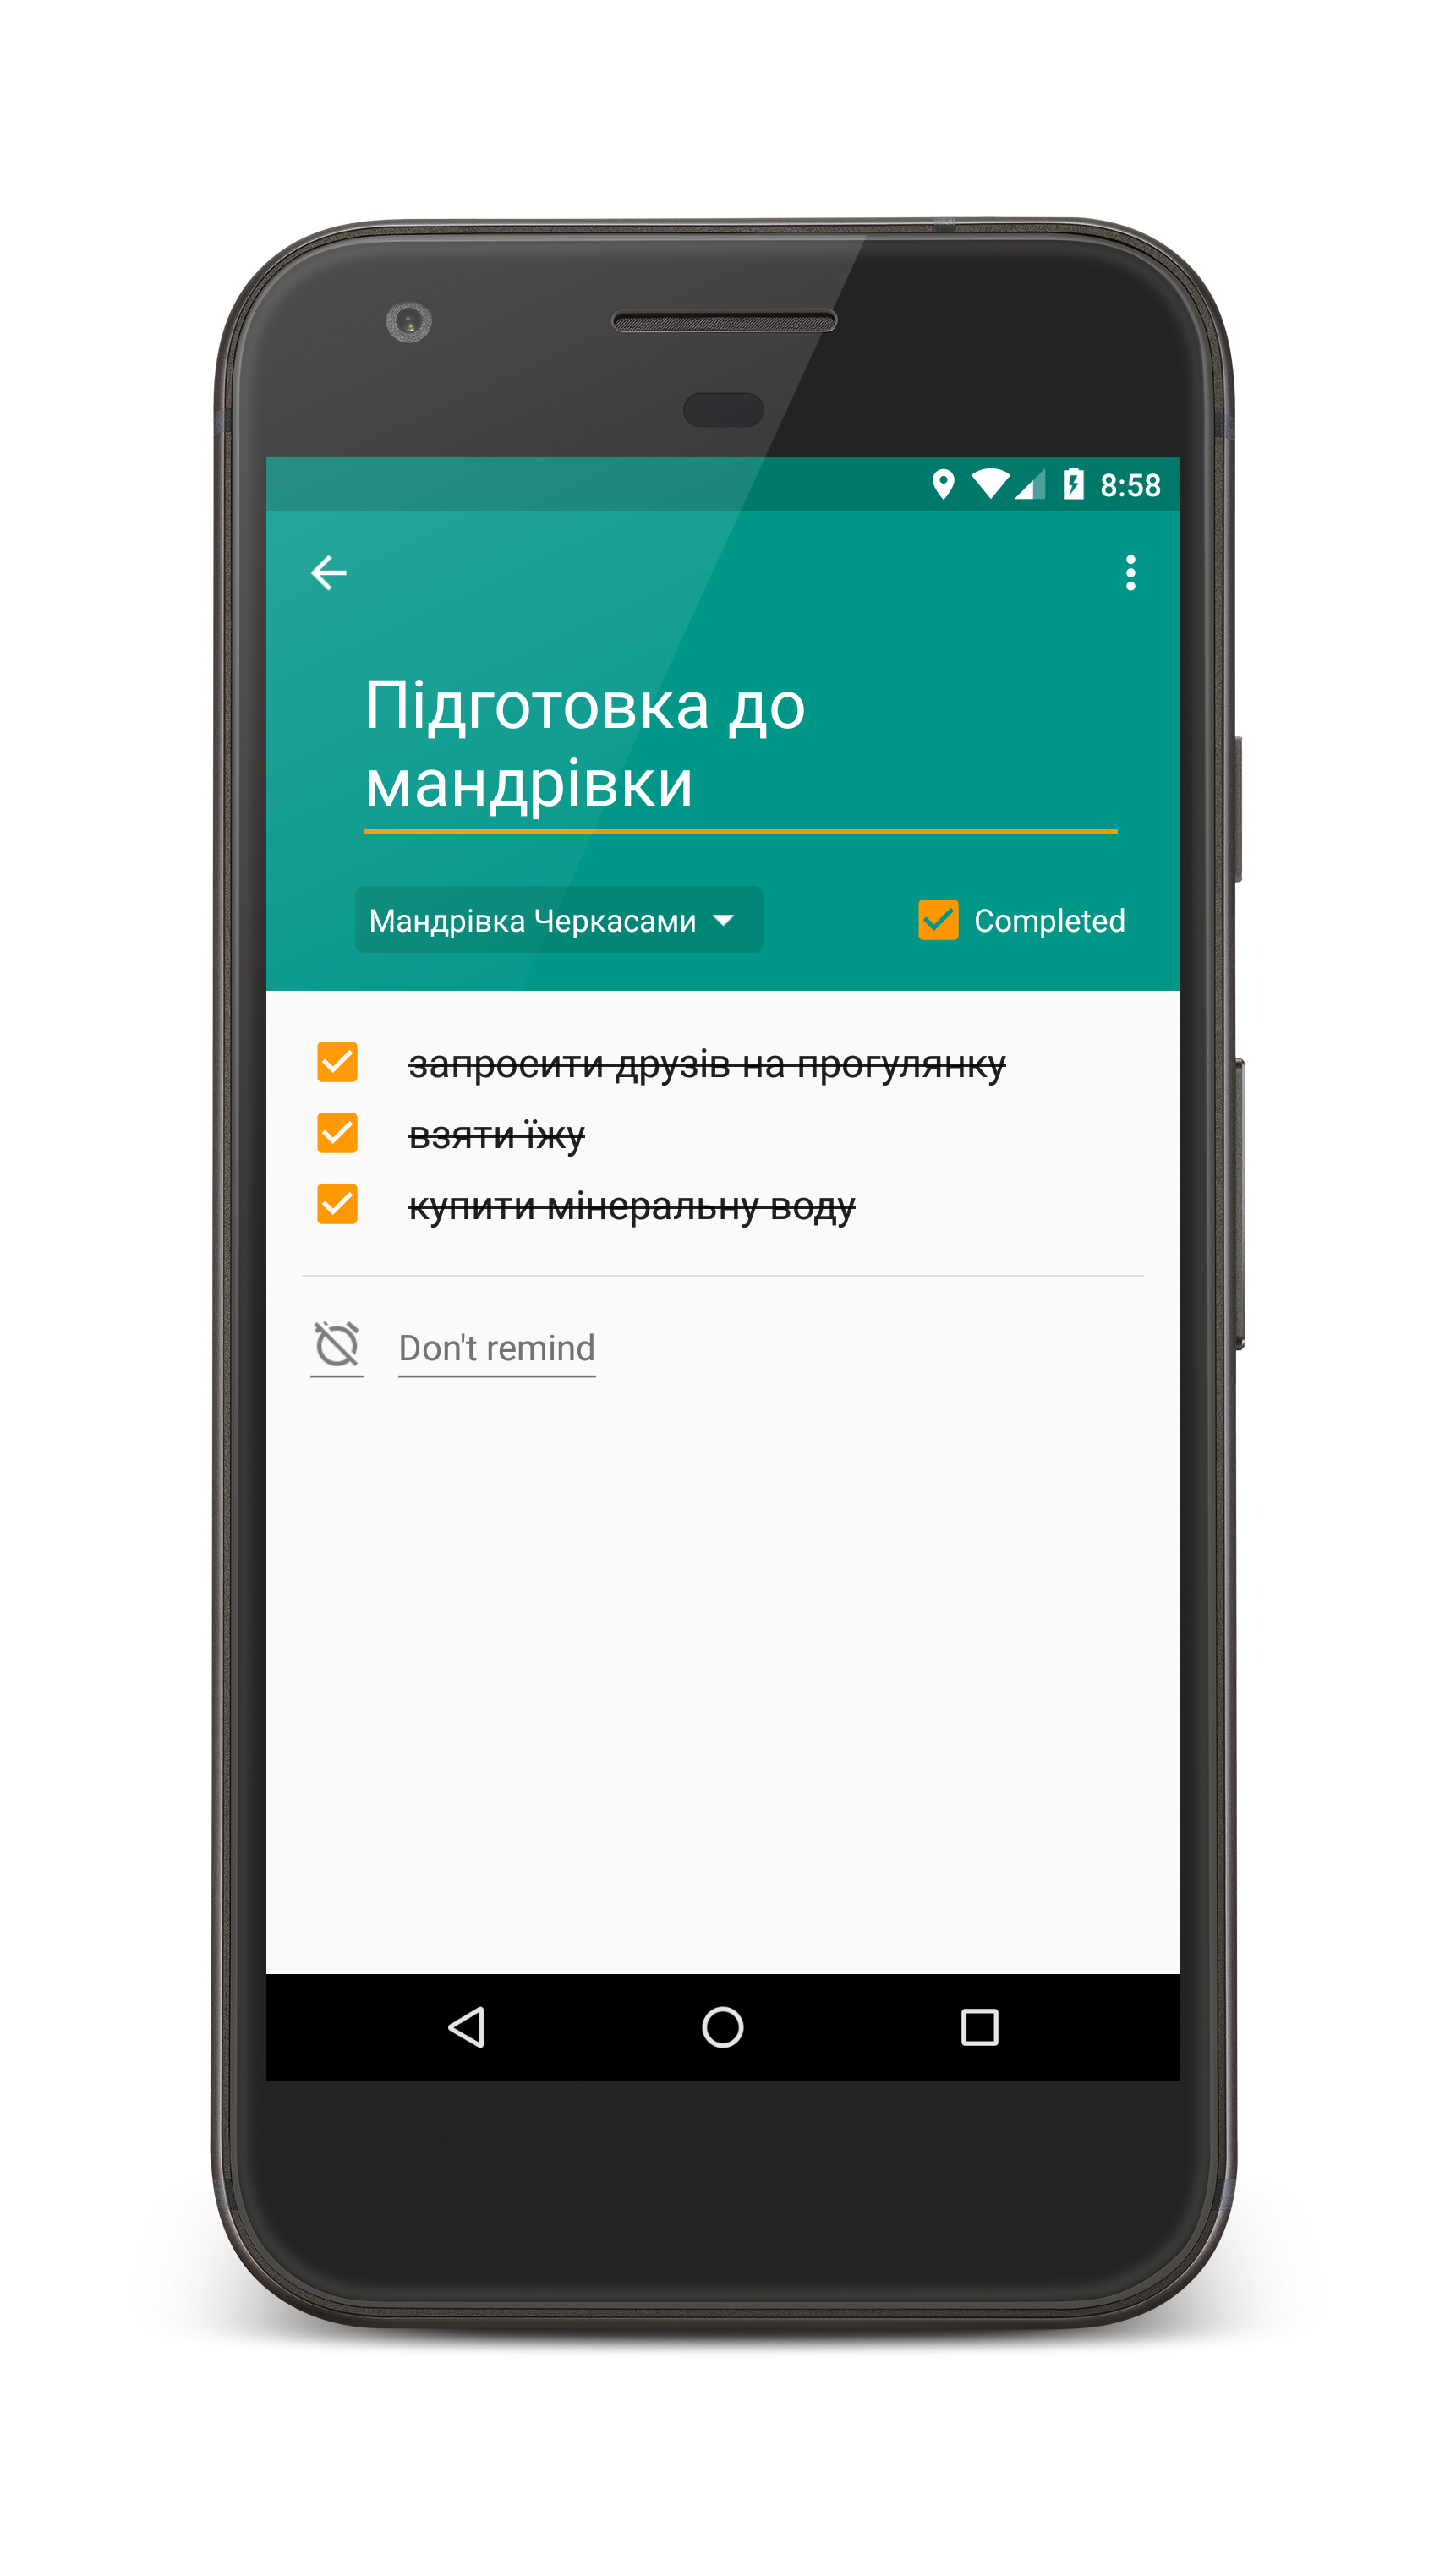
\includegraphics[width=0.75\textwidth]{reminderitem_screen}
	\caption{Екран запису планувальника}
	\label{reminder_screen}
\end{figure}

\begin{figure}[H]
	\centering
	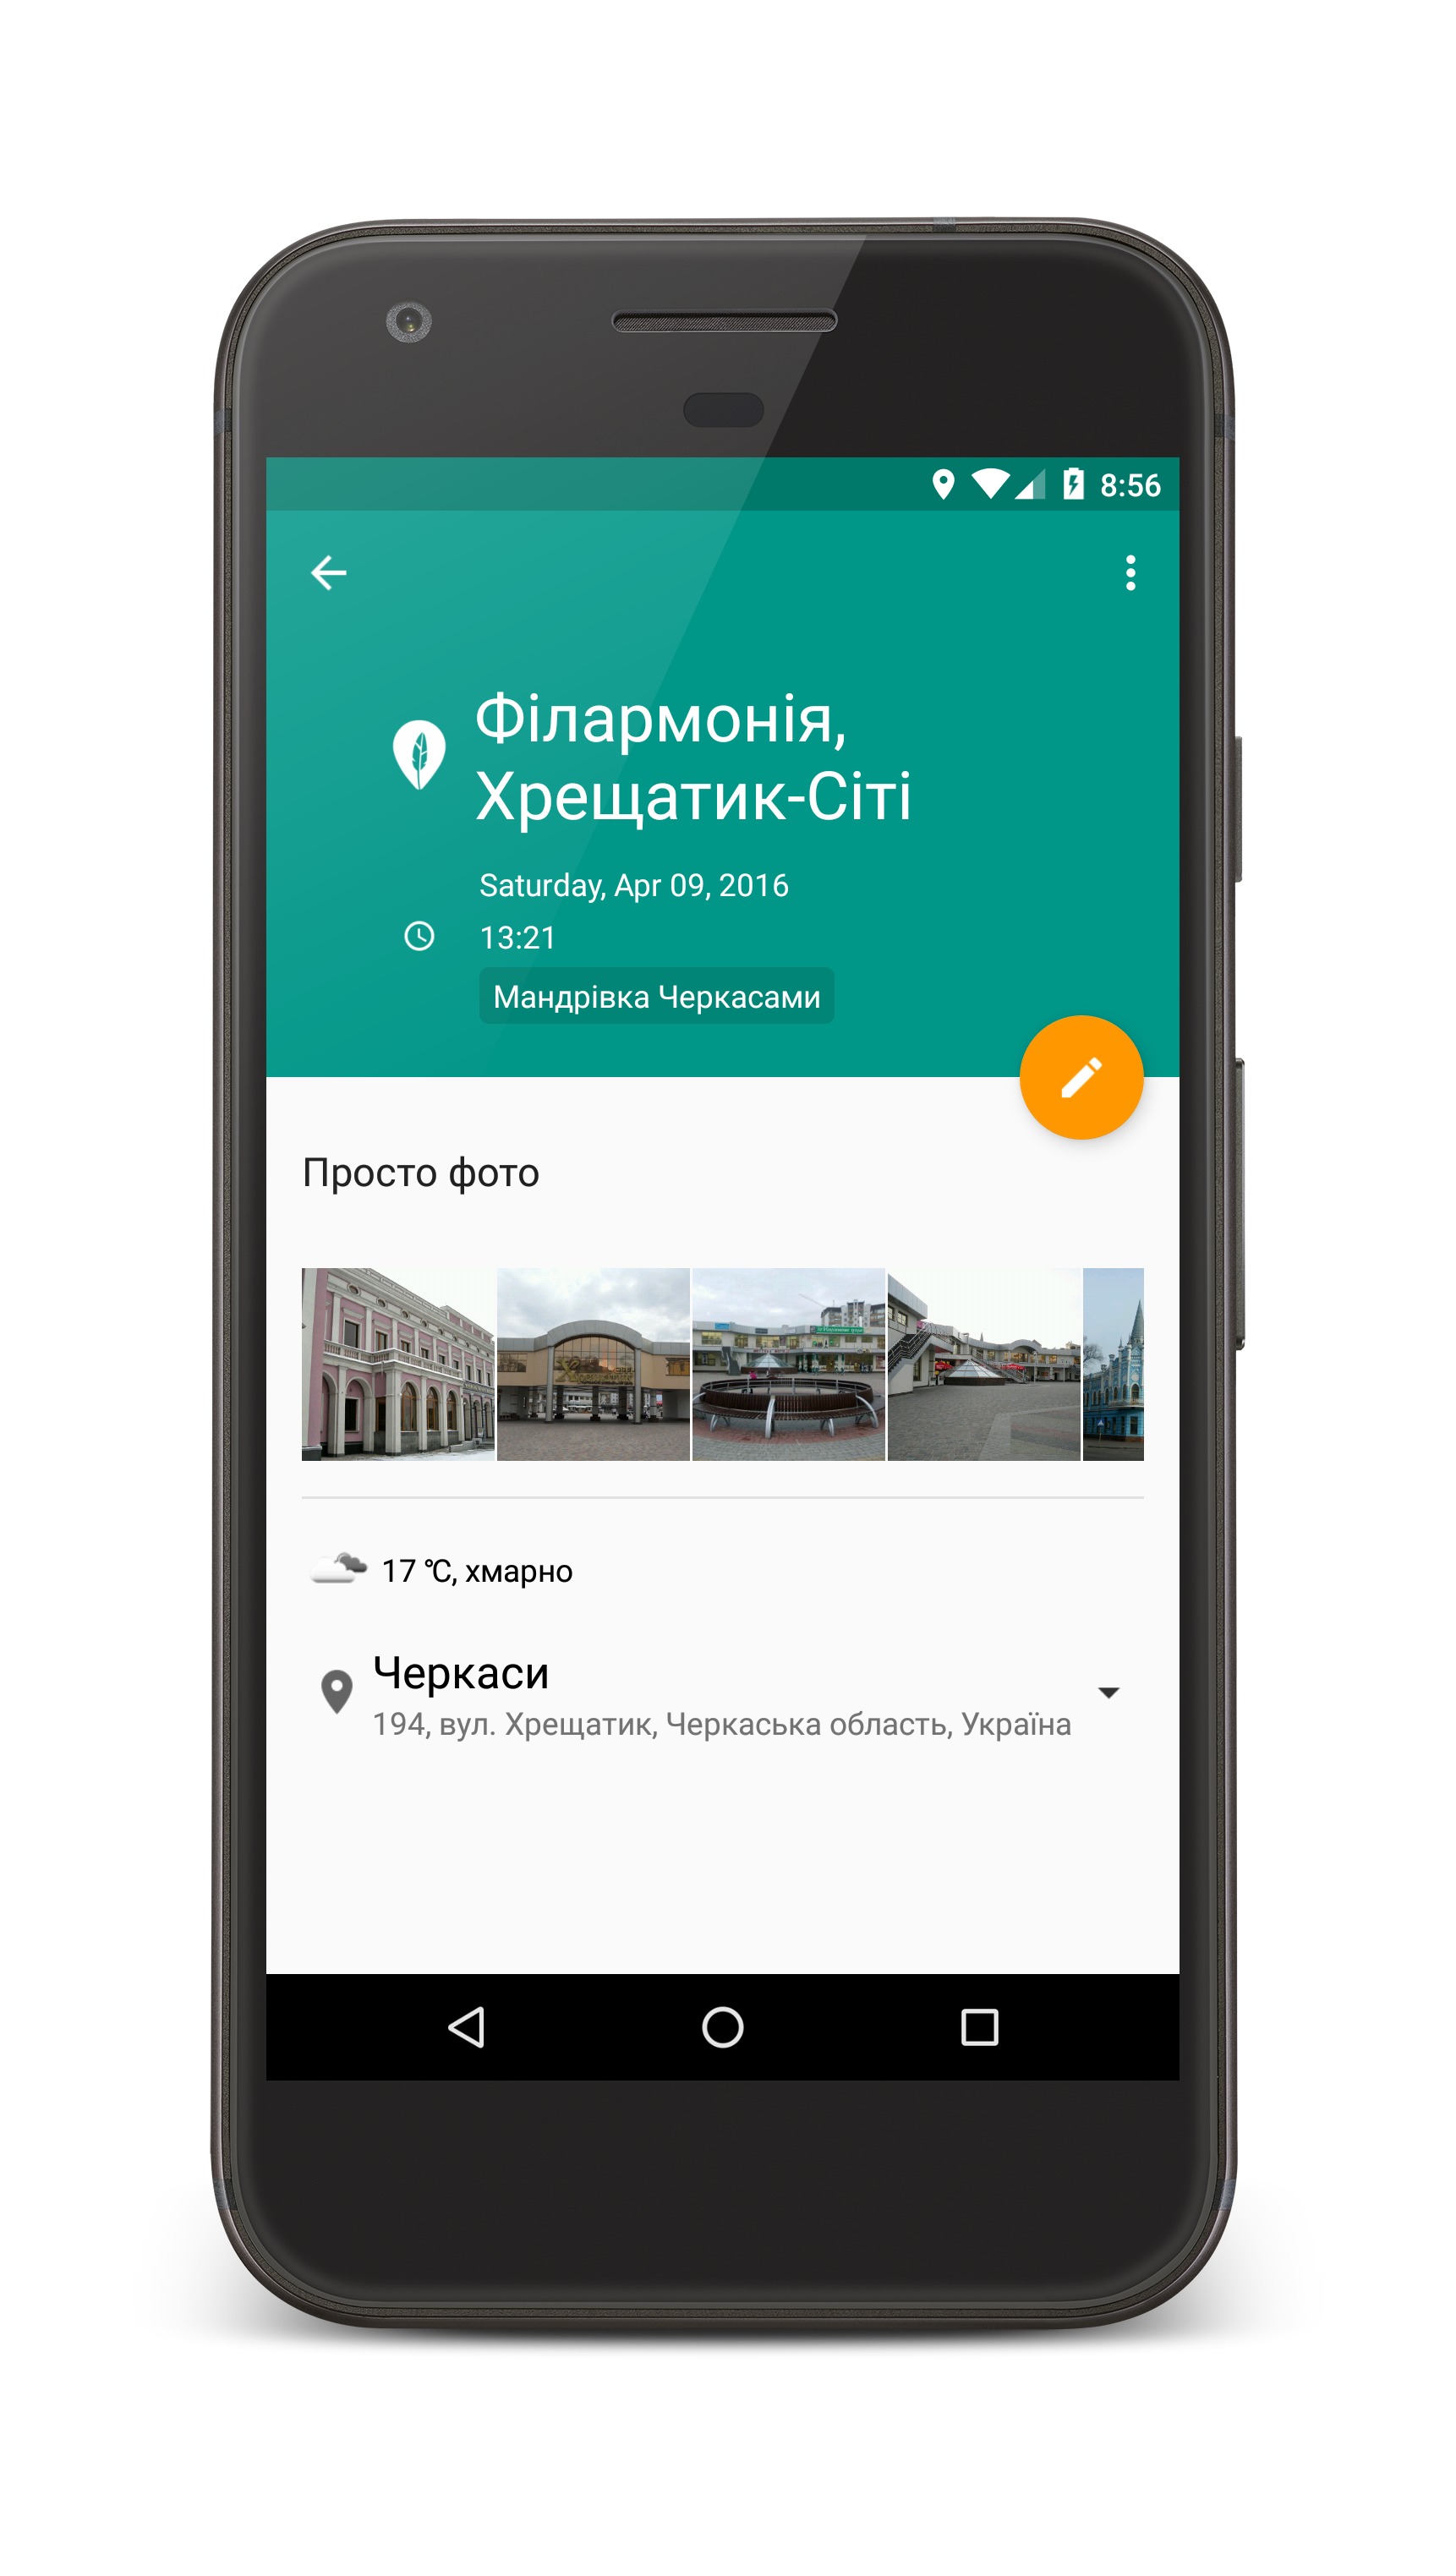
\includegraphics[width=0.75\textwidth]{diarynote_screen}
	\caption{Екран запису щоденника}
	\label{diary_screen}
\end{figure}

\begin{figure}[H]
	\centering
	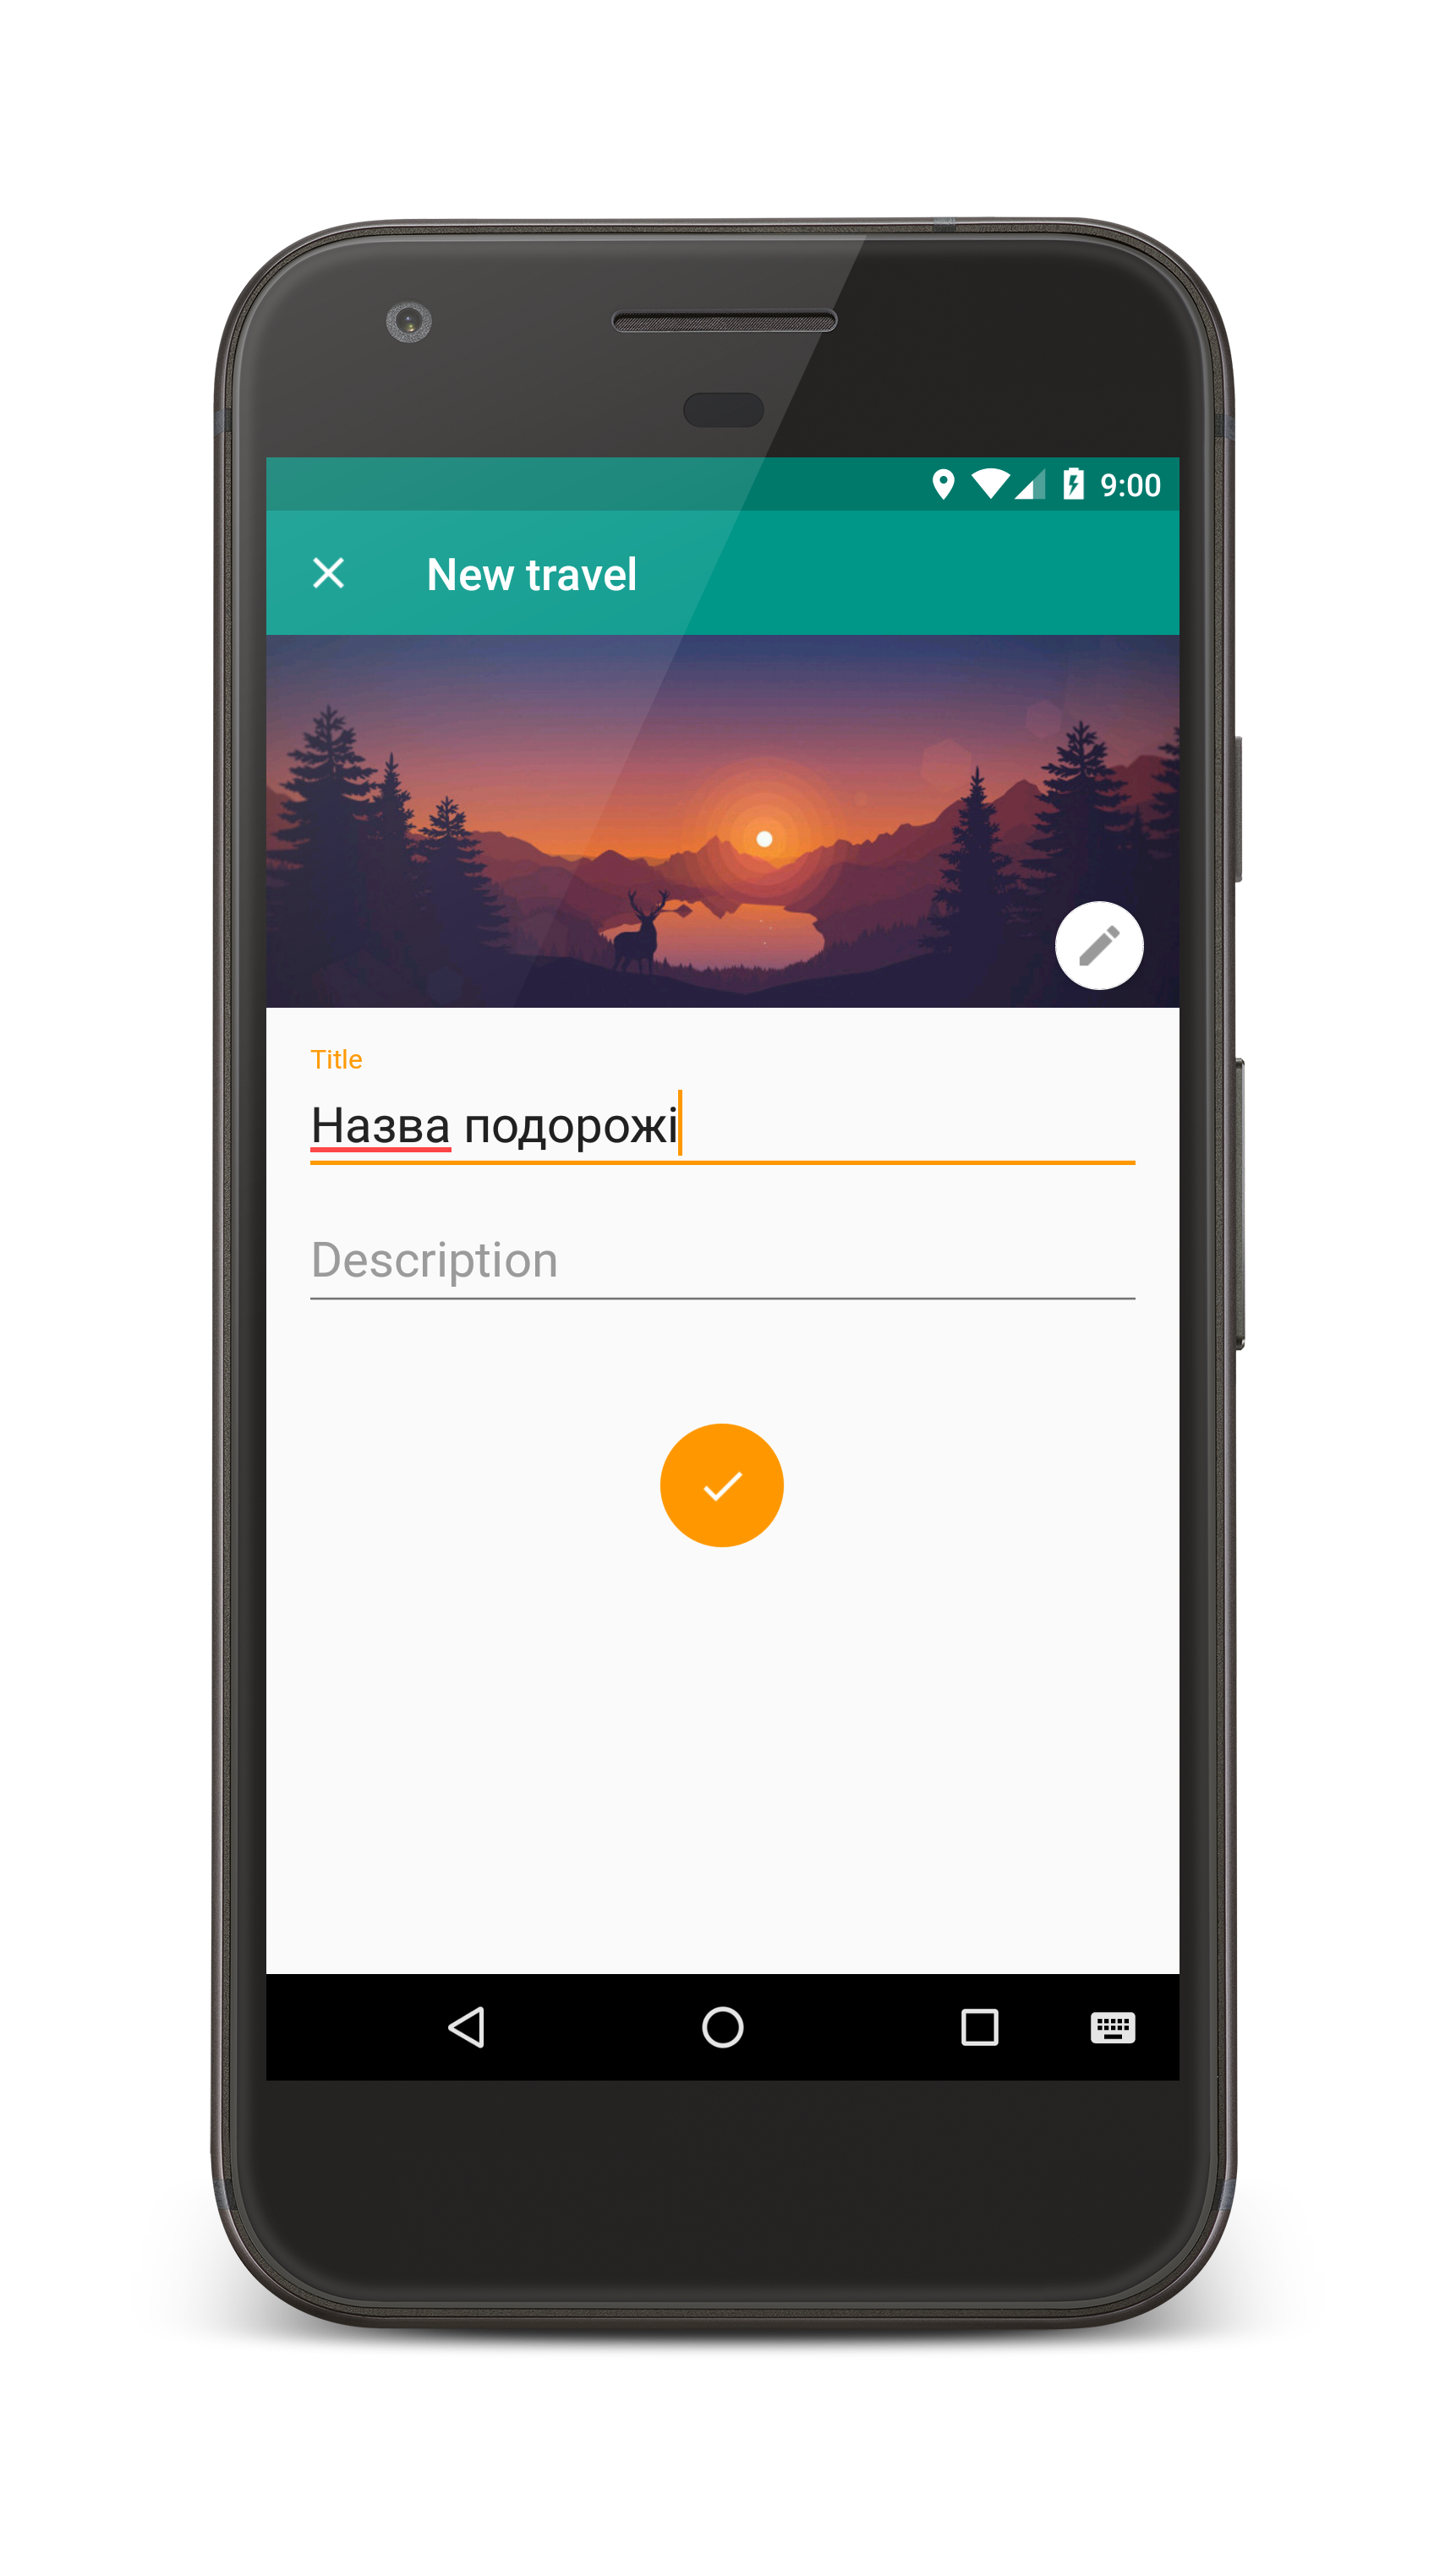
\includegraphics[width=0.75\textwidth]{newtravel_screen}
	\caption{Екран створення/редагування подорожі}
	\label{new_travel_screen}
\end{figure}

\begin{figure}[H]
	\centering
	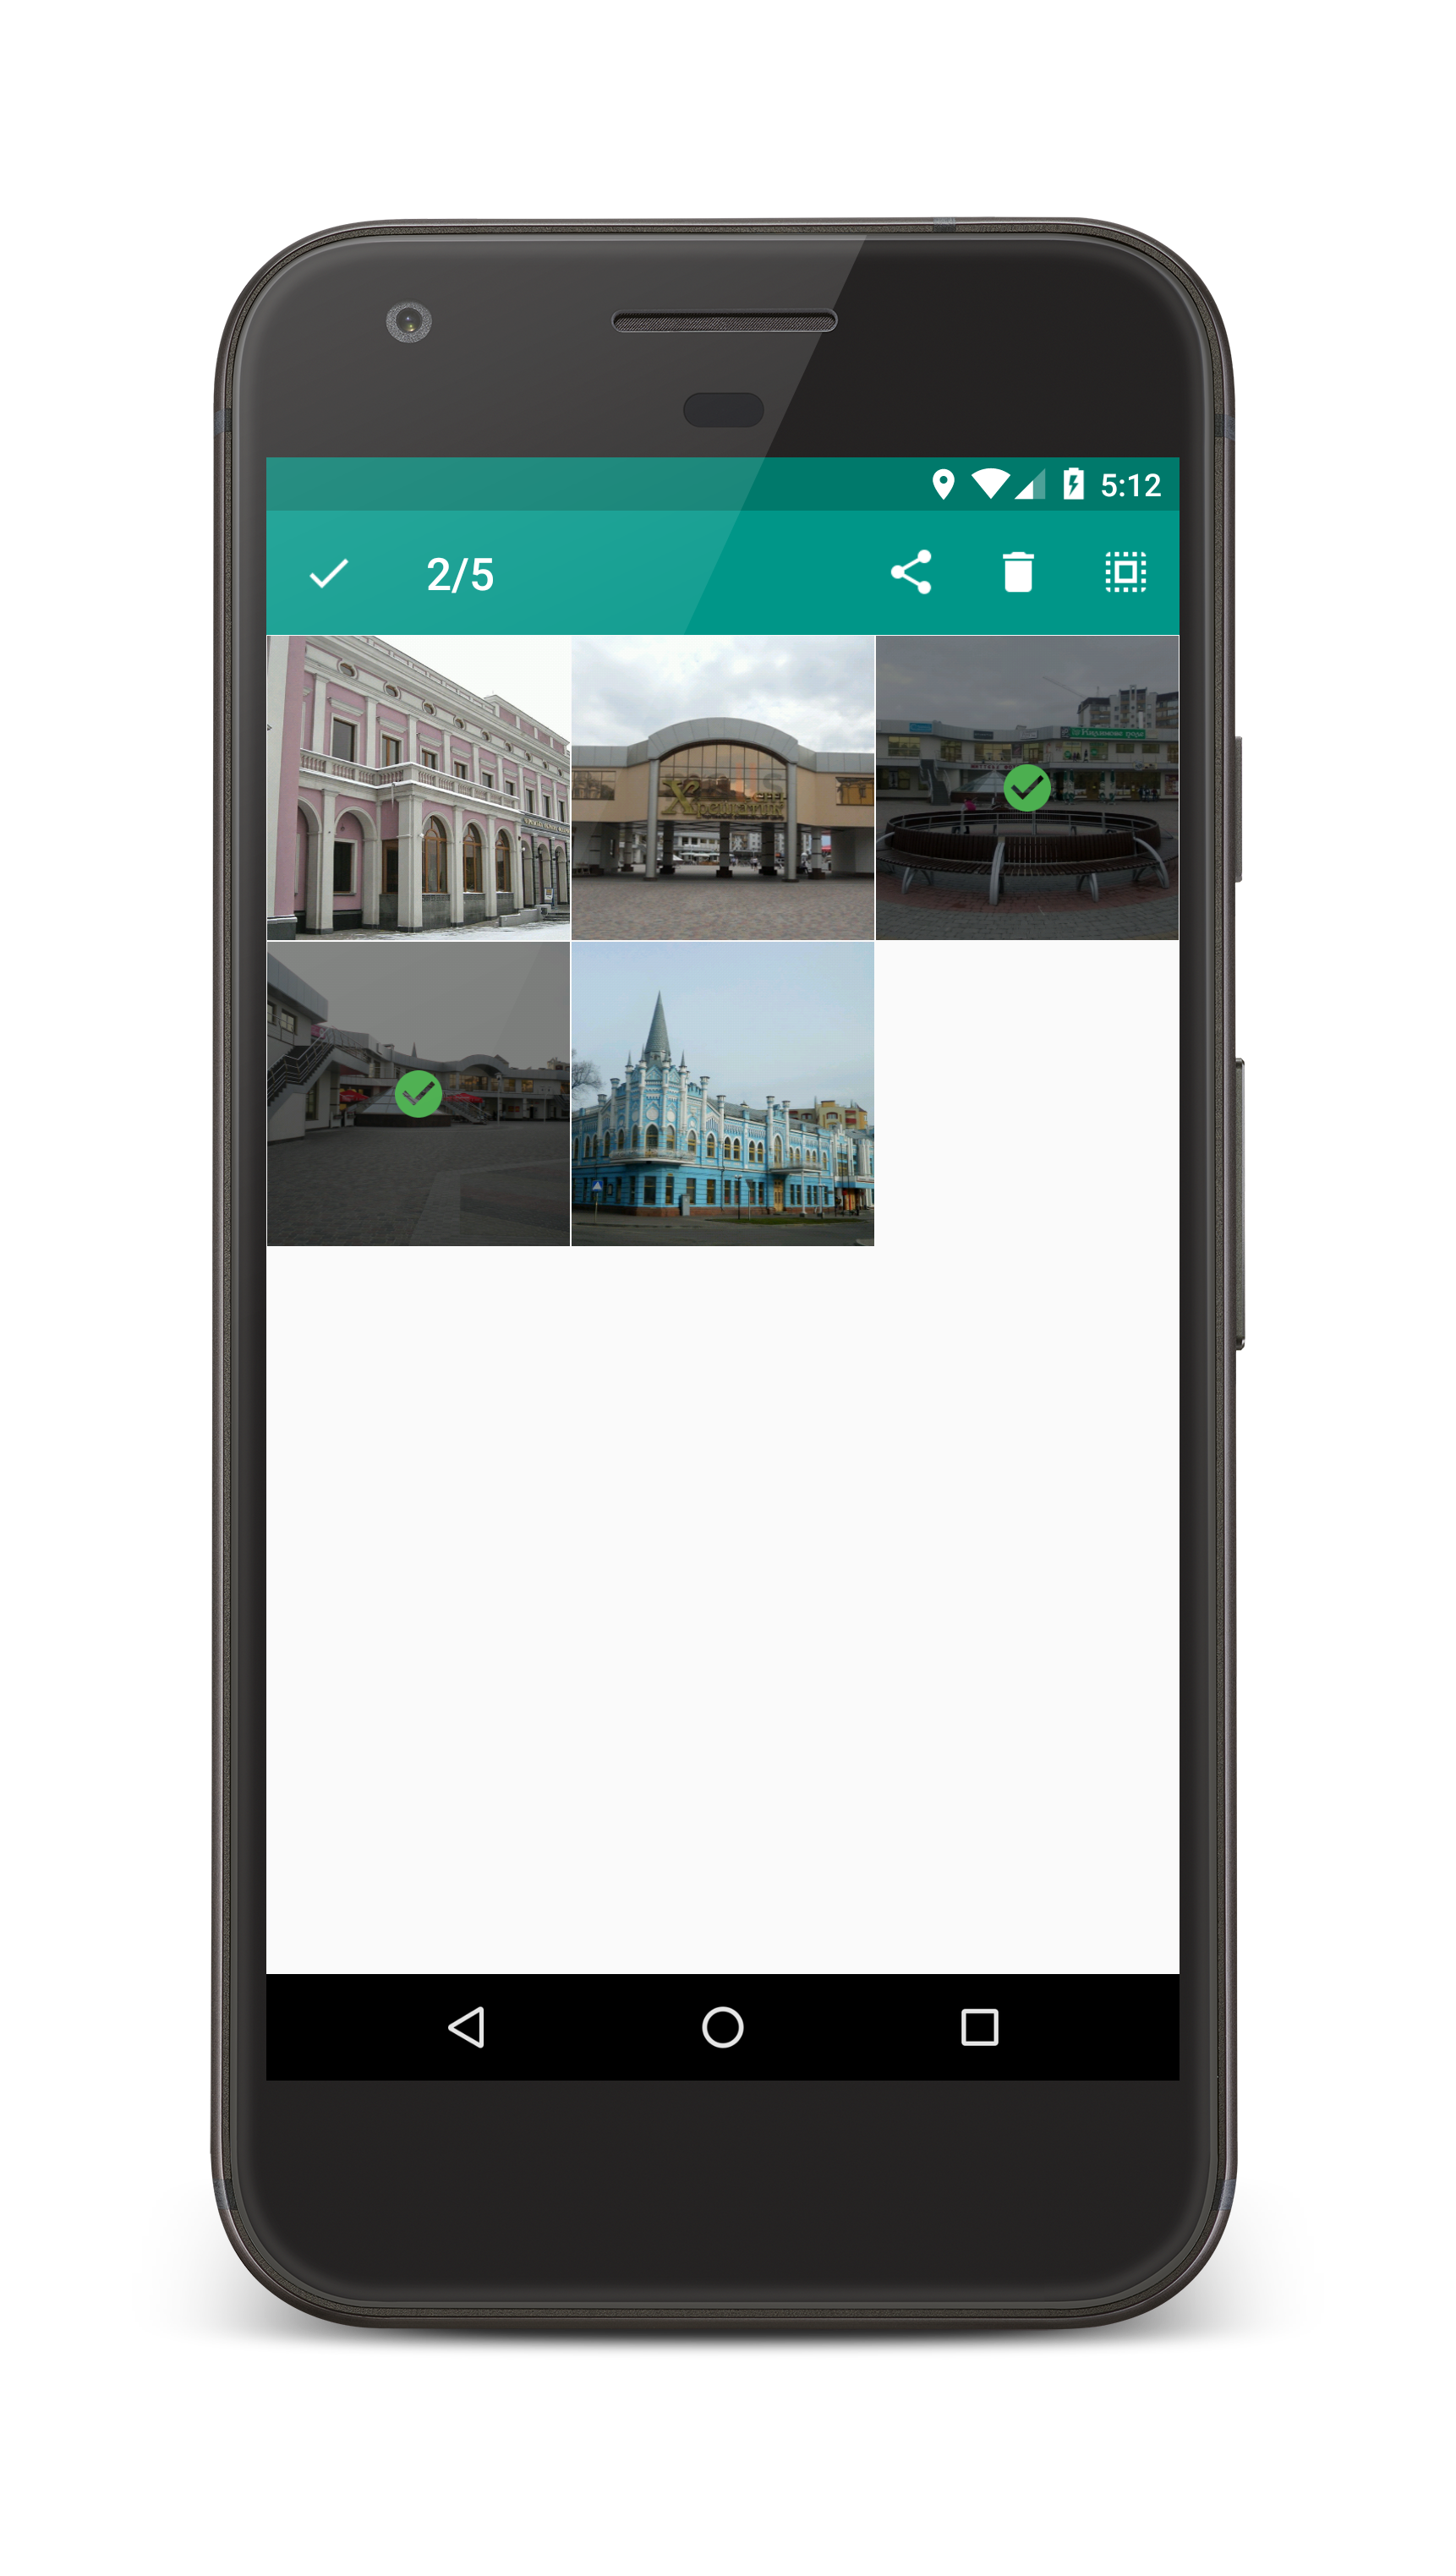
\includegraphics[width=0.75\textwidth]{images_screen}
	\caption{Екран списку фотографій у записі щоденника}
	\label{photo_screen}
\end{figure}

\newpage
\section*{Додаток Б}\addcontentsline{toc}{section}{Додаток Б}
\begin{center}
	\bfseries Текст програми
\end{center}

\begin{center}
	(знаходиться на оптичному диску)
\end{center}